%%%%%%%%%%%%%%%%%%%%%%%%%%
\documentclass[12pt]{article} 
\usepackage{setspace} %line spaces
\setstretch{2}
\usepackage[a4paper, margin=2.5 cm]{geometry} % margin on JEB authors guidelines
% spaces between headers
\usepackage[raggedright]{titlesec} %raggedright option = don't cut titles!
% MS Word style justification rather than latex-style hyphenation
\tolerance=1
\emergencystretch=\maxdimen
\hyphenpenalty=10000
\hbadness=10000
\usepackage{graphicx} % for graphics
\usepackage{float} % to position graphics
\usepackage[labelfont=bf]{caption} % for caption
%\usepackage[font={color=gray}]{caption}
\captionsetup[figure]{font={stretch=1.2}}    %% change 1.2 as you like

\usepackage{fontspec}
\setmainfont{Arial}
% colors section
\usepackage[dvipsnames]{xcolor}
\definecolor{navyblue}{RGB}{14, 53, 179}
\definecolor{coolblack}{rgb}{0.0, 0.18, 0.39} %citations color
\usepackage{soul}% highlighting color
\sethlcolor{green}
%\hyphenchar\font=-1 %stop hyphenation
\usepackage[hyphens]{url}
\usepackage{hyperref}%for DOI & reset subsections
\hypersetup{colorlinks,linkcolor=black,urlcolor=navyblue,citecolor=navyblue} 
\setlength{\parindent}{0pt} % no paragraph indentation
\setlength{\parskip}{1em} %but a space
\usepackage{textcomp} % provides underscore
%bibliography:
\usepackage[style=apa,backend=biber,maxcitenames=2,natbib=true,url=false, uniquename=false, uniquelist=false]{biblatex}
\usepackage[british]{babel}
\usepackage{csquotes}
\DeclareLanguageMapping{british}{british-apa}
\LetLtxMacro{\cite}{\citet}  % year in ()

% mode d'emploi:
%\citep{venables_modern_2002} \par
%\cite{kahle_ggmap_2013-1}
%\parencite[e.g.][trucapres]{venables_modern_2002, kahle_ggmap_2013-1}

% so that the title for the bibliography section is not "bibliography" but "references"
\DefineBibliographyStrings{english}{%
  bibliography = {References},
}

%awesome explanation for generating (a) and (b) same author, same year but not same coauthors list. In summary, use uniquelist=false and force manually bibtex entry with sortyear and sortname. https://tex.stackexchange.com/questions/251285/biblatex-same-first-author-same-year-cite-as-a-b-etc

% so that initials of authors dont appear in the text.use uniquename=false https://tex.stackexchange.com/questions/134535/biblatex-authoryear-style-in-text-citations-display-first-name-initials-for-ce

% so that all authors are cited in the reference list (such as Boissy et al. 2007)
\renewcommand{\maxprtauth}{99}

% maybe "no issue" could work using biber (I also used that for other styles to tell biblatex not to read the ISBN or ISSN...)
\DeclareSourcemap{
  \maps[datatype=bibtex]{
    \map{
      \step[fieldset=number, null]
    }
  }
}
%YEAH! it worked <3
\addbibresource{PhDthesis2305.bib}

%for not having 5 authors cited in the text:https://tex.stackexchange.com/questions/452032/setting-maxcitenames-for-biblatex-apa

%combined with this: https://tex.stackexchange.com/questions/97031/how-to-modify-apa-biblatex-style-to-look-like-elsarticle-harv-style

\makeatletter
\newcommand{\apamaxcitenames}{8}

\DeclareNameFormat{labelname}{%
  % First set the truncation point
  \ifthenelse{\value{uniquelist}>1}
    {\numdef\cbx@min{\value{uniquelist}}}
    {\numdef\cbx@min{\value{minnames}}}%
  % Always print the first name and the second if there are only two since
  % "et al" must always be plural
  \ifboolexpr{test {\ifnumcomp{\value{listcount}}{=}{1}}
              or test {\ifnumcomp{\value{listtotal}}{=}{2}}}
    {\usebibmacro{labelname:doname}%
      {\namepartfamily}%
      {\namepartfamilyi}%
      {\namepartgiven}%
      {\namepartgiveni}%
      {\namepartprefix}%
      {\namepartprefixi}%
      {\namepartsuffix}%
      {\namepartsuffixi}}
    % We are looking at name >=3
    % If the list is 6 or more names or we have seen citation before, potential truncation
    {\ifboolexpr{test {\ifnumcomp{\value{listtotal}}{>}{\value{maxnames}}}
                 or test {\ifciteseen}}
     % Less than the truncation point, print normally
     {\ifnumcomp{\value{listcount}}{<}{\cbx@min + 1}
       {\usebibmacro{labelname:doname}%
         {\namepartfamily}%
         {\namepartfamilyi}%
         {\namepartgiven}%
         {\namepartgiveni}%
         {\namepartprefix}%
         {\namepartprefixi}%
         {\namepartsuffix}%
         {\namepartsuffixi}}
       {}%
      % At potential truncation point ...
      \ifnumcomp{\value{listcount}}{=}{\cbx@min + 1}
        % but enforce plurality of et al - only truncate here if there is at
        % least one more element after the current potential truncation point
        % so that "et al" covers at least two elements.
        {\ifnumcomp{\value{listcount}}{<}{\value{listtotal}}
          {\printdelim{andothersdelim}\bibstring{andothers}}
          {\usebibmacro{labelname:doname}%
            {\namepartfamily}%
            {\namepartfamilyi}%
            {\namepartgiven}%
            {\namepartgiveni}%
            {\namepartprefix}%
            {\namepartprefixi}%
            {\namepartsuffix}%
            {\namepartsuffixi}}}
        {}%
      % After truncation point, do not print name
      \ifnumcomp{\value{listcount}}{>}{\cbx@min + 1}
       {\relax}%
       {}}%
     % We are looking at name >=3
     % Name list is < 6 names or we haven't seen this citation before, print normally
     {\usebibmacro{labelname:doname}%
       {\namepartfamily}%
       {\namepartfamilyi}%
       {\namepartgiven}%
       {\namepartgiveni}%
       {\namepartprefix}%
       {\namepartprefixi}%
       {\namepartsuffix}%
       {\namepartsuffixi}}}}
\makeatother

\usepackage{etoolbox}  % or xpatch

\bibliography{mybib.bib}
\def\bibfont{\footnotesize}
\usepackage{lineno} %linenumbers
\linenumbers
\renewcommand\linenumberfont{\normalfont\small}
%%% titles
\titlespacing*\section{0pt}{0pt}{0pt}
\titlespacing*\subsection{0pt}{0pt}{0pt}
% spacing: how to read {12pt plus 4pt minus 2pt}, 12pt is what we would like the spacing to be
%           plus 4pt means that TeX can stretch it by at most 4pt,  minus 2pt means that TeX can shrink it by at most 2pt
%       This is one example of the concept of, 'glue', in TeX
%number only from subsections on
\usepackage{chngcntr}
\counterwithout{subsection}{section}
\usepackage{titlesec}% with a point
\titlelabel{\thetitle.\quad}
\titleformat*{\section}{\large\bfseries}
\usepackage{upgreek} % greek letters not in italic upalpha etc.

%%%% for BiorXiv
\usepackage{authblk}
\title{Coupling between tolerance and resistance differs between related \textit{Eimeria} parasite species: implications for coevolution with their mouse hosts}
\author[1,2]{Alice Balard}  
\author[1,2]{Víctor Hugo Jarquín-Díaz}
\author[1]{Jenny Jost}
\author[1]{Vivian Mittné}
\author[1]{Francisca Böhning}
\author[3]{Ľudovít Ďureje}
\author[3]{Jaroslav Piálek}
\author[1,2]{Emanuel Heitlinger}
\affil[1]{Institute for Biology. Department of Molecular Parasitology. Humboldt University Berlin (HU). Philippstr. 13, Haus 14, 10115, Berlin, Germany}
\affil[2]{Leibniz-Institut für Zoo- und Wildtierforschung (IZW) im Forschungsverbund Berlin e.V.. Alfred-Kowalke-Straße 17, 10315, Berlin, Germany}
\affil[3]{Research Facility Studenec, Institute of Vertebrate Biology, Czech Academy of Sciences, Květná 8, 603 65 Brno, Czech Republic}
\date{}                     %% if you don't need date to appear
\setcounter{Maxaffil}{0}
\renewcommand\Affilfont{\itshape\small}
\setlength{\affilsep}{.3em}%between authors and affil

\makeatletter
\def\@maketitle{%
  \newpage
  \null
  \vskip 2em%
  \begin{center}%
    \let \footnote \thanks
         {\large\textbf \@title \par}%
         \vskip 1.5em%
                {\small
                  \lineskip .5em%
                  \begin{tabular}[t]{c}%
                    \baselineskip=12pt
                    \@author
                  \end{tabular}\par}%
                \vskip 1em%
                       {\large \@date}%
  \end{center}%
  \par
  \vskip -3em}
\makeatother

%%%%%%%%%%%%%%%%%%%% Document code starts here %%%%%%%%%%%%%%%%%%%%
\begin{document}

{\let\clearpage\relax%
  \maketitle }

\textbf{Corresponding author:} Alice Balard, alice.cam.balard@gmail.com\\
\textbf{Authors contributions:} AB, JP and EH designed the experiment and analysis. LD and JP provided the research material. AB, VHJD, JJ, VM and FB carried out the experiment. AB performed the analysis. AB and EH wrote the manuscript, with major contribution from JP and feedback from all the authors.
Funding: This work was funded by the German Research Foundation (DFG) Grant [HE 7320/1-1] to EH. VHJ is an associated student of GRK 2046 funded by the DFG. The maintenance of wild-derived strains was supported by the ROSE program from Czech Academy of Sciences and the Czech Science Foundation (project 16-23773S) to JP. \\
\textbf{Data accessibility:} Code and data used for this article can be found at: \href{https://github.com/alicebalard/Article_RelatedParasitesResTol}{https://github.com/alicebalard/Article\_RelatedParasitesResTol}

\section*{Abstract}
Resistance (host capacity to reduce parasite burden) and tolerance (host capacity to reduce impact on its health for a given parasite burden) manifest two different lines of defence. Tolerance can be independent from resistance, traded-off against it, or the two can be positively correlated because of redundancy in underlying (immune) processes. We here tested whether this coupling between tolerance and resistance could differ upon infection with closely related parasite species.
We tested this in experimental infections with two parasite species of genus \textit{Eimeria}. We measured proxies for resistance (the (inverse of) number of parasite transmission stages (oocysts) per gram of feces at the day of maximal shedding) and tolerance (the slope of maximum relative weight loss compared to day of infection on number of oocysts per gram of feces at the day of maximal shedding for each host strain) in four inbred mouse strains and four groups of F1 hybrids belonging to two mouse subspecies, \textit{Mus~musculus~domesticus} and \textit{M.~m.~musculus}. We found a negative correlation between resistance and tolerance against \textit{E.~falciformis}, while the two are uncoupled against \textit{E.~ferrisi.} We conclude that resistance and tolerance against the first parasite species might be traded off, but evolve more independently in different mouse genotypes against the latter. We argue that evolution of the host immune defences can be studied largely irrespective of parasite isolates if resistance-tolerance coupling is absent or weak (\textit{E.~ferrisi}) but host-parasite coevolution is more likely observable and best studied in a system with negatively correlated tolerance and resistance (\textit{E.~falciformis}).

\textbf{Keywords}: Resistance, Tolerance, \textit{Eimeria}, Coevolution

\section*{Introduction}

Host defence mechanisms evolve to alleviate the detrimental effect of parasites. They can be categorised into two components: resistance and tolerance \citep{raaberg_decomposing_2009}. Resistance is the ability of a host to reduce parasite burden, resulting from defence against parasite infection or proliferation early after infection \citep{schmid-hempel_evolutionary_2013}. The negative effect of resistance on parasite fitness can lead to antagonistic coevolution. According to theoretical models, fluctuating host and parasite genotypes arise, and balancing selection maintains resistance alleles polymorphic \citep{Boots2008, roy_evolutionary_2000}. Resistance has been the classical "catch all" measure for host-parasite systems, but recently it has been shown to be incomplete, especially with respect to potential fitness effects on the host \citep{kutzer_maximising_2016, raaberg_decomposing_2009}.\par

Disease tolerance \parencite[not to be confused from "immunological tolerance", unresponsiveness to self antigens;][]{medzhitov_disease_2012} is the ability of the host to limit the impact of parasite on its fitness \citep{raaberg_decomposing_2009, Vale2012, kutzer_maximising_2016}. By potentially providing a longer-living niche, this defence mechanism improves, or at least does not deteriorate, the fitness of the parasite. Tolerance alleles are thus predicted by theoretical models to evolve to fixation due to positive feedback loops \citep{Boots2008, restif_concurrent_2004, roy_evolutionary_2000}. From a mechanistic perspective tolerance alleviates direct or indirect damage \parencite[e.g. excessive immune response underlying resistance against parasites, called immunopathology;][]{graham_evolutionary_2005} caused by parasites \citep{raaberg_decomposing_2009}. Tolerance mechanisms include modulation of inflammatory response \citep{Ayres2012}, tissue repair \parencite[stress response, damage repair and cellular regeneration mechanisms;][]{soares_disease_2017}, and compensation of parasite-induced damage by increase of reproductive effort \citep{Baucom2011}. The resulting metabolic costs of resistance and tolerance, with and without parasite infection, determine the optimal (steady state and infection inducible) extent and of both immune defences \citep{sheldon_ecological_1996}.\par

Resistance and tolerance can be positively associated if they involve the same metabolic pathway, as was shown in the plant model \textit{Arabidopsis thaliana} in response against herbivory \citep{mesa_molecular_2017}. In animals, genetic association studies of resistance and tolerance of \textit{Drosophila melanogaster} against the bacterium \textit{Providencia rettgeri} have shown positively correlated genetic effects, as the same loci were associated with changes of both traits in the same direction \citep{howick_genetic_2017}.\par

Nevertheless, resistance and tolerance can also be genetically and physiologically independent, involving different proximate mechanisms. Lack of correlation between both defences was shown for example in monarch butterflies (\textit{Danaus plexippus}) infected by the protozoan parasite \textit{Ophryocystis elektroscirrha}. This study found genetic variation in resistance between butterflies families, but a fixed tolerance \citep{Lefvre2010}. Similarly, no correlation could be found between resistance and tolerance for the fish \textit{Leuciscus burdigalensis} in response to infection with its parasite \textit{Tracheliastes polycolpus}. The authors explain the decoupling of both defences by the fact that, in this system, tolerance likely involves wound repair rather than immune regulation, making resistance and tolerance mechanisms independent \citep{MazGuilmo2014}.\par

Eventually, in other systems, resistance and tolerance have been found negatively correlated. For examples, inbred laboratory mouse strains lose weight upon infection with \textit{Plasmodium chabaudi.} The extent of this impact on host health is negatively correlated with the peak number of parasites found in the blood \citep{raaberg_disentangling_2007}, meaning that mouse strains with higher resistance present lower tolerance. Similarly, infections of sea trout (\textit{Salmo trutta trutta}) and Atlantic salmon (\textit{Salmo salar}) with the trematode \textit{Diplostomum pseudospathaceum} showed that resistance and tolerance were negatively correlated when assessing mean levels of both traits in different host populations \citep{klemme_vertebrate_2016}. This is interpreted as a result of trade-off between resistance and tolerance \citep{sheldon_ecological_1996, restif_concurrent_2004, raaberg_decomposing_2009}.\par

We have seen that depending on the system studied resistance and tolerance can be (1) uncoupled (independent), (2) positively correlated (involving same genes and mechanisms), or (3) negatively correlated (traded-off). Theoretical models show that coupling between resistance and tolerance (or absence thereof) could depend not only on the host but also on the parasite \citep{Carval2010}. Here we tested this hypothesis. More precisely, we asked whether there could be differences in the resistance-tolerance coupling upon infection of one host type with two closely related parasite species. To answer this question, we infected four inbred mouse strains and four groups of F1 hybrids representative of two house mouse subspecies, \textit{M.~m.~domesticus} and \textit{M.~m.~musculus}, with three parasite isolates representative of two naturally occuring parasite species, the protozoan parasite \textit{Eimeria ferrisi} and \textit{E.~falciformis }\citep{jarquin-diaz_detection_2019}. \textit{Eimeria }spp. are monoxenous parasites that expand asexually and reproduce sexually in intestinal epithelial cells, leading to malabsorption of nutrients, tissue damage and weight loss \citep{chapman_chapter_2013}. The evolutionary history of these different \textit{Eimeria} species in the two house mouse subspecies is unknown and it is unclear whether subspecies-specific adaptation exists in one or the other. 

\par
We tested if coupling between resistance and tolerance differs between both parasite species and discussed the implication for parasite-host coevolution. Additionally, as coevolving hosts and parasites can adapt to their antagonist, we tested adaptation to the host subspecies (hereafter "host adaptation") of \textit{E.~ferrisi} to \textit{Mus~musculus}, using a parasite isolated in a \textit{M.~m.~domesticus} host and one in a \textit{M.~m.~musculus} host. Higher parasite fitness of one isolate in one of the two hosts and inversely for the second isolate, or higher host fitness upon infection with one of the two parasite isolates and inversely for the second isolate, would be indirect evidence for coevolution of this parasite with \textit{Mus~musculus}. 

\section*{Material and methods}

\subsection{Parasite isolates}

The three parasite isolates used in this study were isolated from feces of three different \textit{M.~m.~domesticus/M.~m.~musculus} hybrid mice captured in Brandenburg, Germany, in 2016 (capture permit No. 2347/35/2014). The parasite isolates belong to both the most prevalent \textit{Eimeria }species in this area, namely \textit{E.~ferrisi }(isolates Brandenburg64 and Brandenburg139) and \textit{E.~falciformis }(isolate Brandenburg88)\citep{jarquin-diaz_detection_2019}. Isolate Brandenburg64 was isolated in a 92\% \textit{M.~m.~domesticus} individual (hybrid index (HI) = 0.08: Proportion of \textit{M.~m.~musculus} alleles in a set of 14 diagnostic markers, see \cite{Balard2020}), isolate Brandenburg139 in a 85\% \textit{M.~m.~musculus} (HI=0.85) and isolate Brandenburg88 in a 80\% \textit{M.~m.~domesticus} (HI=0.2). Pre-patency and the peak day of parasite shedding for these isolates were estimated during infection in NMRI laboratory mice \citep{al-khlifeh_eimeria_2019} which were also used for serial passaging of the isolates. Parasite infective forms (oocysts) were recovered by flotation in saturated NaCl solution followed by washing and observation under light microscope (following the protocol described in \cite{clerc_parasitic_2019}) and stored at room temperature in 1mL of 2\% potassium dichromate for a maximum of 2 months before infection of the wild-derived mice. Oocysts were allowed to sporulate 10 days before infection in a water bath at 30$^{\circ}$C.\par

\subsection{Mouse groups}

We used four wild-derived inbred mouse strains from which we generated four groups of F1 hybrids. Two parental strains represented \textit{M.~m.~domesticus}: \textbf{SCHUNT} (Locality: Schweben, Hessen, Germany [N: 50$ ^{\circ} $ 26’, E: 9$ ^{\circ} $ 36’] \citep{martincova_phenotypic_2019}) and \textbf{STRA} (Locality: Straas, Bavaria, Germany [N: 50$ ^{\circ} $ 11’, E: 11$ ^{\circ} $ 46’] \citep{pialek_development_2008}, and two derived from \textit{M.~m.~musculus}: \textbf{BUSNA} (Locality: Buškovice, Bohemia, Czech Republic [N: 50$ ^{\circ} $ 14’, E: 13$ ^{\circ} $ 22’] \citep{pialek_development_2008}) and \textbf{PWD} (Locality: Kunratice, Bohemia, Czech Republic [N: 50$ ^{\circ} $ 01’, E: 14$ ^{\circ} $ 29’] \citep{gregorova_pwdph_2000}). The four groups of F1 hybrids consisted of two intrasubspecific hybrids (\textbf{SCHUNTxSTRA }and \textbf{PWDxBUSNA}) and two intersubspecific hybrids (\textbf{STRAxBUSNA} and \textbf{SCHUNTxPWD})(\textbf{Figure 1}). Age of the mice at the time of infection ranged between 5.6 and 21.4 weeks. All mouse strains and F1 hybrids were obtained from the Institute of Vertebrate Biology of the Czech Academy of Sciences in Studenec (licence number 61974/2017-MZE-17214; for further details on strains see \url{https://housemice.cz/en}).\par

Parasites of the \textit{Eimeria }genus are known to induce host immune protection against reinfection \citep{rose_immune_1992, smith_genetic_2000}. To ensure that our mice were \textit{Eimeria}-naive, mouse fecal samples were tested before infection for the presence of \textit{Eimeria }spp. oocysts by flotation in saturated NaCl solution followed by washing and observation under light microscope. \par

\subsection{Experimental infection}

Mice were kept in individual cages during infection. Water and food (SNIFF, Rat/Mouse maintenance feed 10 mm) were provided \textit{ad libitum} supplemented with 1 g of sunflower and barley seeds per day. Mice were orally infected with 150 sporulated oocysts of one \textit{Eimeria }isolate suspended in 100$\mu$l phosphate-buffer saline (PBS) and monitored daily until their sacrifice by cervical dislocation at time of regression of infection (reduction of oocyst output). Individuals presenting severe health deficiency and/or a weight loss approaching 18\% relative to their starting weight were sacrificed earlier at defined humane end points (experiment license Reg. 0431/17). Weight was recorded and feces collected on a daily basis. Fecal pellets were collected every day from each individual cage and suspended in 2\% potassium dichromate. Parasite oocysts were recovered using NaCl flotation (see above). \par

All individuals were negative for \textit{Eimeria }at the beginning of our experiment (before infection of first batch, as described in the next paragraph). In total, 168 mice were infected. Mice were randomly allocated to experimental groups ensuring homogeneous distribution of ages and sexes between groups. Our experiments were conducted in four (partially overlapping) consecutive batches for logistical reasons. The first two batches were infected with the two \textit{E.~ferrisi }isolates (Brandenburg64 and Brandenburg139), the third and fourth by one \textit{E.~ferrisi }isolate (Brandenburg64) and one \textit{E.~falciformis }isolate (Brandenburg88). Our experimental design is summarized in \textbf{Table 1} (chronology of experimental batches can be scrutinized in \textbf{Supplementary Table S1}). \par

Nematode infection is common in breeding facilities (Baker, 1998) and could interact with \textit{Eimeria} \citep{clerc_parasitic_2019}. We surveyed for their presence and nematode eggs were observed in flotated feces of mice belonging to all genotypes before the experiment. Despite treatment of the first infection batch of mice (B1, 22 mice) with anthelminthics (Profender®, Bayer AG, Levekusen, Germany) following the protocole of Mehlhorn et al. (2005), nematodes were still detected with PCR (following the protocole of \cite{floyd_nematode-specific_2005}) in randomly sampled fecal samples a week later. We therefore decided not to treat mice of the following infection batches. Moreover, we observed \textit{Eimeria }oocysts in the feces of 28 mice belonging to the last experimental batch (batch B4) at the day of infection, likely due to cross-contamination between batches. For following statistical analyses, we considered along with the full data set (N=168) a conservative data set in which cross-contaminated animals and animals treated by anthelminthic were removed (N=118). Results obtained on the conservative data set can be found in \textbf{Supplementary Material S2}. Despite differences in significance due to a lower statistical power, the main conclusions of our analyses were consistent with those obtained on the main data set.\par

\subsection{Statistical analyses}

\subsubsection{Choice of proxies for resistance, impact of parasite on host and tolerance}
As resistance is the capacity of a host to reduce its parasite burden, it is usually estimated by the inverse of infection intensity \citep{raaberg_decomposing_2009}. Pre-patency (the time to shedding of infectious stages, so called oocysts) is longer for \textit{E.~falciformis} (7 days) than for \textit{E.~ferrisi} (5 days) \citep{al-khlifeh_eimeria_2019}. Therefore, as a proxy of (inverse of) resistance we used the number of oocysts per gram of feces (OPG) at the day of maximal shedding. Using the Spearman's non-parametric rank correlation test, we found this measurement to be tightly correlated with the sum of oocysts shed throughout the experiment (Spearman's $\uprho$=0.93, N=168, P<0.001). Due to the aggregation characteristic of parasites \citep{shaw_patterns_1995}, the appropriate distribution for maximum number of OPG was found to be the negative binomial distribution. This was confirmed based on log likelihood, AIC criteria and goodness-of-fits plots (density, CDF, Q-Q, P-P plots; R packages MASS \citep{venables_modern_2002} and fitdistrplus \citep{delignette-muller_fitdistrplus_2015}). \par

Both parasite species provoke inflammation, cellular infiltration, enteric lesions, diarrhea, and ultimately weight loss \citep{ankrom_life_1975, ehret_dual_2017, schito_comparison_1996, al-khlifeh_eimeria_2019}. Therefore, the impact of parasites on host health was measured as the maximum relative weight loss compared to day 0 (body weight measured at the start of the experimental infection). For mice sacrificed at humane end points before the end of the experiment, last weight of the living animal was used. This weight (loss) can be expected to be a very conservative estimate for our analyses (rendering tolerance conservatively low for these animals, which might have lost more weight if not sacrificed). \par

Tolerance is usually defined as a reaction norm, i.e. the regression slope of host fitness (or health condition if that is the parameter of interest) on infection intensity per host genotype \citep{Simms2000, raaberg_decomposing_2009}. Thus tolerance was assessed as the slope of maximum relative weight loss compared to day 0 on number of OPG at the day of maximal shedding, within each mouse group and for each parasite isolate. A steep slope indicates a low tolerance (high weight lost for a given parasite burden).

\subsubsection{Statistical modelling}

Maximum OPG and relative weight loss were modelled separately as a response of either mouse group, parasite isolate and their interaction. We used a negative binomial generalised linear model for maximum OPG, and a linear model for relative weight loss. For tolerance, we performed a linear regression with null intercept (as each mouse was controlled against itself at start of the experiment, before losing weight or shedding parasite), modelling relative weight loss as a response of maximum OPG interacting either mouse group, parasite isolate and their interaction. To test the significance of the marginal contribution of each parameter to the full model, each parameter was removed from the full model, and the difference between full and reduced model was assessed using likelihood ratio tests (G). \par

For each of our model, we also asked within each parasite isolate if the response differed between mouse groups using likelihood ratio tests (G) as described above. Of note, four mice infected by\textit{E.~falciformis} isolate Brandenburg88 did not shed any oocysts as death occurred at or one day before the peak of oocysts shedding in other mice. For this reason, we modelled maximum OPG for mice infected with this parasite using a zero-inflated negative binomial (ZINB) generalised linear model, after verifying that it provided a better fit than the simple negative binomial based on log likelihood and AIC criteria.\par

\subsubsection{Test of host adaptation}

Host adaptation of \textit{E.~ferrisi} was tested using two isolates (the "Western" Brandenburg64 and "Eastern" Brandenburg139) and our four parental mouse strains (the two \textit{M.~m.~domesticus} Western SCHUNT and STRA, and the two \textit{M.~m.~musculus }Eastern BUSNA and PWD). We hypothesised a possible host adaptation of \textit{E.~ferrisi}. The prediction drawn from this would be that the Eastern parasite (\textit{E.~ferrisi} isolate Brandenburg139) reproduces better in the matching Eastern mouse subspecies (\textit{M.~m.~musculus}) than in the Western one (\textit{M.~m.~domesticus}), and similarly the Western parasite (\textit{E.~ferrisi} isolate Brandenburg64) reproduce better in \textit{M.~m.~domesticus} than in \textit{M.~m.~musculus.} Additionally, a higher tolerance of each host infected by its matching parasite despite similar parasite reproductive output could indicate increased host fitness, and host adaptation.\par

\subsubsection{Test of coupling between resistance and tolerance}

We tested coupling between resistance and tolerance for \textit{E.~ferrisi} and \textit{E.~falciformis }using the isolates Brandenburg64 and Brandenburg88 and our eight mouse groups. To test such coupling, one can assess the strength of correlation between measure of resistance and measure of tolerance \citep{raaberg_disentangling_2007}. Of note, tolerance (in absolute value) is measured as the slope $\upalpha$ of the linear regression of parasite load (x) on maximum relative weight loss (y) of equation y = $\upalpha$ x + $\upbeta$ ($\upalpha$ being the slope and $\upbeta$ the intercept, 0 in our case). Therefore, tolerance is expressed as $\upalpha$ = y/x – $\upbeta$/x. As x and y/x are by definition not independent, testing the correlation between resistance and tolerance can lead to spurious correlation \citep{Brett2004}. To alleviate the dangers of this statistical artifact, we additionally tested differences in resistance, impact on health and tolerance between mouse groups separately and also the underlying correlation between mean parasite load (x) and mean relative weight loss (y). We use the terminology "coupling" (between resistance and tolerance) to describe genotype-level correlation between tolerance and resistance additionally supported by the absence of positive correlation between health-effect and resistance. Correlations were tested using Spearman’s rank correlation.\par

All analyses were performed using R version 3.5.2 \citep{R_2010}(negative binomial: function glm.nb from R package MASS \citep{venables_modern_2002}; ZIBN: function zeroinfl from R package pscl \citep{Jackman2020, Zeileis2008}; linear model: function lm from R core package stats; mean and 95\% confidence intervals: function ggpredict from R package ggeffect \citep{Ldecke2018}). Graphics were produced using the R package ggplot2 \citep{wickham_ggplot2_2016} and compiled using the free software inkscape (\href{https://inkscape.org/}{https://inkscape.org}).
\par

\section*{Results}
\setcounter{subsection}{0}
\renewcommand*{\theHsubsection}{chX.\the\value{subsection}}

\subsection{General}

Parasites of all isolates successfully infected all mouse groups (at the exception of 5 individuals infected by \textit{E.~falciformis} isolate Brandenburg88 that died or had to be sacrificed due to a strong weight loss before the peak of shedding for this parasite), meaning that no "qualitative infection resistance" (\textit{sensu} \cite{Gandon2000}) was detected. For \textit{E.~ferrisi }(both isolates Brandenburg139 and Brandenburg64), the pre-patent period was 5 days post infection (dpi) and the median day of maximal oocyst shedding was 6 dpi (standard deviation sd=0.7 and 0.9, respectively). The median day of maximum weight loss was 5 dpi for both isolates (sd=2.1 and 1.7 respectively). For \textit{E.~falciformis} (isolate Brandenburg88) pre-patency was 7 dpi, median day of maximal shedding was 8 dpi (sd=1.3) and median day of maximal weight loss 9 dpi (sd=1.6)(\textbf{Figure 2}). Of note a considerable number of mice infected with this isolate (13 out of 56 = 23$\%$ ) died or had to be sacrificed at humane end points less than 3 days after the oocysts shedding peak for the group, all belonging to \textit{M.~m.~musculus} subspecies (PWD, BUSNA, or their F1 PWDxBUSNA; 5 died at dpi 8, 5 at dpi 9, 3 at dpi 10). \textit{E.~falciformis }isolate Brandenburg88 was more lethal for the \textit{M.~m.~musculus} mice strains than for the other strains ($\chi_{7}^{2}$= 31.96, P<0.001; \textbf{Table 2}).\par

\subsection{No indication of host adaptation of \textit{E.~ferrisi}}

We tested if our proxies for resistance, impact on weight and tolerance were different between the four parental mouse strains and between both \textit{E.~ferrisi} infection isolates (isolate Brandenburg64 and Brandenburg139). Maximum parasite load differed between mouse strains (LRT: G=25.5, df=6, P<0.001), but the interaction term mouse strain-parasite isolate was non significant (LRT: G=4.1, df=3, P=0.25). A similar result was found for maximum relative weight loss (LRT: mouse strain: G=16.8, df=6, P=0.01; interaction mouse strain-parasite isolate: G=4.1, df=3, P=0.25). This indicates that when resistance and impact on weight vary between host strains, they do so independently of the parasite isolate. Eventually, the variables mouse strain, parasite isolate and their interaction were found non significant at the 0.05 threshold for the slope of the linear regression between the two, indicating that differences of tolerance could not be detected between mouse strains or parasite isolates (\textbf{Figure 3}). Our results do not indicate either (1) an increased reproduction of each parasite in its matching host or (2) a higher tolerance of host infected by its matching parasite despite similar parasite reproductive output. Thus they do not support the hypothesis of host adaptation between \textit{E.~ferrisi} and its host.

\subsection{Resistance and tolerance to \textit{E.~ferrisi }isolate Brandenburg64 are uncoupled}

We tested coupling between resistance and tolerance for \textit{E.~ferrisi} isolate Brandenburg64 in our eight mouse groups. First, we tested whether our proxies for resistance, impact on weight and tolerance were different between the mouse groups. We found the maximum number of OPG and relative weight loss to be statistically different between mouse groups (LRT: maximum number of OPG: G=26.6, df=7, P<0.001; \textbf{Figure 4A}; maximum relative weight loss: G=21.5, df=7, P<0.01; \textbf{Figure 4B}). Tolerance was not found to significantly differ between mouse groups for this parasite isolate (LRT: G=6.8, df=7, P=0.45; \textbf{Figure 4C}).\par

We found a non significant positive correlation between resistance (inverse of maximum number of OPG) and impact on health (maximum weight loss) (Spearman's $\uprho$=0.69, P=0.07, N=8; \textbf{Figure 4D}). Eventually, we did not find a correlation between resistance (inverse of maximum number of OPG) and tolerance (inverse of slope of maximum weight loss on maximum OPG) (Spearman's $\uprho$=0, P=1, N=8; \textbf{Figure 4E}). \par

In conclusion, we did not find indications of resistance-tolerance coupling for \textit{E.~ferrisi} isolate Brandenburg64, the different mouse groups infected by this parasite presenting a similar level of tolerance while showing an effect of quantitative resistance on health.\par

\subsection{Coupling between resistance and tolerance to \textit{E.~falciformis}}

We then tested coupling between resistance and tolerance for \textit{E.~falciformis} isolate Brandenburg88 in our eight mouse groups. First, we tested if our proxies for resistance, impact on weight and tolerance were different between the mouse groups. We found the maximum number of OPG and relative weight loss to be statistically different between mouse groups (LRT: maximum number of OPG: G=28.6, df=14, P=0.012; \textbf{Figure 5A}; maximum relative weight loss: G=21, df=7, P<0.01; \textbf{Figure 5B}). Finally, contrary to our results on \textit{E.~ferrisi} isolate Brandenburg64, the tolerance slopes for \textit{E.~falciformis} isolate Brandenburg88 were different between mouse groups (LRT: G=13.9, df=7, P=0.05; \textbf{Figure 5C}).\par

We detected a strong negative correlation between (inverse of) resistance (maximum number of OPG) and tolerance (inverse of slope of maximum weight loss on maximum OPG) (Spearman's $\uprho$=-0.95, P=0.001; \textbf{Figure 5E}). We conclude that this correlation is unlikely a statistical artifact, as (1) mouse groups present statistically different values of resistance and tolerance and (2) we found a (non significant) negative correlation between resistance (inverse of maximum number of OPG) and impact on health (maximum weight loss) (Spearman's $\uprho$=-0.5, P=0.22; \textbf{Figure 5D}), indicating that mouse groups losing more weight also shed less parasites. \par

We conclude that our results indicate the presence of negative resistance-tolerance coupling for \textit{E.~falciformis} isolate Brandenburg88.

\section*{Discussion}

In this study, we assessed resistance and tolerance to two closely related parasites, \textit{E.~ferrisi} (two isolates) and \textit{E.~falciformis} (one isolate), in four mouse strains and their intra-and intersubspecific hybrids. Understanding this coupling has two major implications. \par

From a practical "measurement" perspective we can ask whether tolerance can be predicted from resistance, as the latter is easier to measure (e.g. in field sampling). Many studies assess the impact of parasites on host fitness based on resistance. If, as we found in the present study, resistance and tolerance are decoupled this can be missleading. In our host system, the house mice, for example, it has been shown that hybrids between \textit{M.~m.~domesticus} and \textit{M.~m.~musculus} are more resistant to parasites \citep{baird_where_2012, Balard2020}, including \textit{Eimeria}, but tolerance could not be measured under natural conditions \citep{Balard2020}. The effect of parasites on host fitness in the evolution of the house mouse hybrid zone is thus still rather ambiguous \citep{baird_shifting_2019}. We show that careful distinction between parasite species is necessary when analysing parasite host interaction \parencite[see also][]{jarquin-diaz_detection_2019} and that it is indispensable to measure both resistance and tolerance in \textit{Eimeria} infections of house mice. \par

In this work we used the concept of tolerance as used originally in the plant litterature \mbox{\citep{Fineblum1995}} and later on transfered to animal studies \mbox{\citep{raaberg_disentangling_2007}}. This concept of tolerance can be criticised, as it links mathematically tolerance to resistance. Nevertheless, we argue that this view is biologically meaningfull considering resistance and tolerance as a step-wise defence system, one step limiting the parasite multiplication, the other limiting the impact of this multiplication on fitness-related traits. To limit the possible statistical artifact, our approch did not only consist in calculing blindly correlations between resistance and tolerance, but we also tested differences in resistance, impact on health and tolerance. We additionally excluded the possibility of positive correlation between mean health-effect and mean resistance of each host strains, which could indicate some host strains having few parasites-few effects on health, and others more parasites-more effects on health: this configuration would limi the possibility of detecting an actual resistance-tolerance trade-off.
\par

More generally, in a evolutionary perspective, coupling between resistance and tolerance might help determine if coevolution between host and parasite can be expected: a host-parasite system in which one finds negative coupling between tolerance and resistance would be an especially promising system for studies of host-parasite co-evolution. Indeed, coevolution in host-parasite systems is often assumed but rarely proven \citep{Woolhouse2002}. \cite{Janzen1980} notes that not all parasite-host systems are coevolving. The presence of efficient host defences against a given parasite is not necessarily produced in response to this parasite specifically and the parasite does not necessarily respond specifically. In the mouse-\textit{E.~ferrisi} system, where resistance and tolerance are decoupled, host and parasite fitness might be decoupled as a result, making host-parasite coevolution less likely. In the mouse-\textit{E.~falciformis} system we found a negative coupling between tolerance and resistance, making coevolution between host and parasite more likely. \par

Differences between parasite species could explain the evolution of different strategies: \textit{E.~ferrisi} commits to sexual reproduction after a relatively short time with few cycles of asexual expansion \citep{al-khlifeh_eimeria_2019, ankrom_life_1975}, while \textit{E.~falciformis} has a relatively longer life cycle \citep{al-khlifeh_eimeria_2019, haberkorn_entwicklung_1970}. As \textit{E.~ferrisi }infections do not reach extremely high intensities, high tolerance might be the optimal strategy for both house mouse subspecies. Resistance could then evolve relatively freely without any major impact of the parasite on the hosts’ health. Moreover, our results did not support host adaptation of \textit{E.~ferrisi}, which might be explained by the absence of host-parasite coevolution caused by uncoupling of parasite and host fitness. In the case of \textit{E.~falciformis}, the long life cycle might lead to high tissue load. Tissue damage is observed during sexual reproduction for this parasite \citep{ehret_dual_2017} and might mean that a certain level of resistance is required. On the other hand, immunopathology has been observed in advanced \textit{E.~falciformis} infections \citep{stange_il-22_2012}. These intrinsic characteristics of \textit{E.~falciformis} might lead to multiple different optima for resistance and tolerance, leading to a trade-off.\par

In conclusion, we argue that the difference between resistance and tolerance coupling in two different parasites can guide research in the house mouse system: if the effects of host hybridisation should be studied independently of potential host-parasite coadaptation, a parasite species leading to uncoupling between resistance and tolerance of the host (e.g. \textit{E.~ferrisi}) might be the most suitable parasite. If coevolution between hosts and parasites should be studied, a parasite species for which resistance and tolerance of the host are negatively correlated (e.g. \textit{E.~falciformis}) would be a more plausible target. Generally, we showed that the coupling between resistance and tolerance can differ between closely related parasite species and we
 argue that this trait of a host-parasite system determines the questions to be best approached with a particular parasite. 

\printbibliography

\section*{Tables}

\begin{figure}[H]
	\centering
	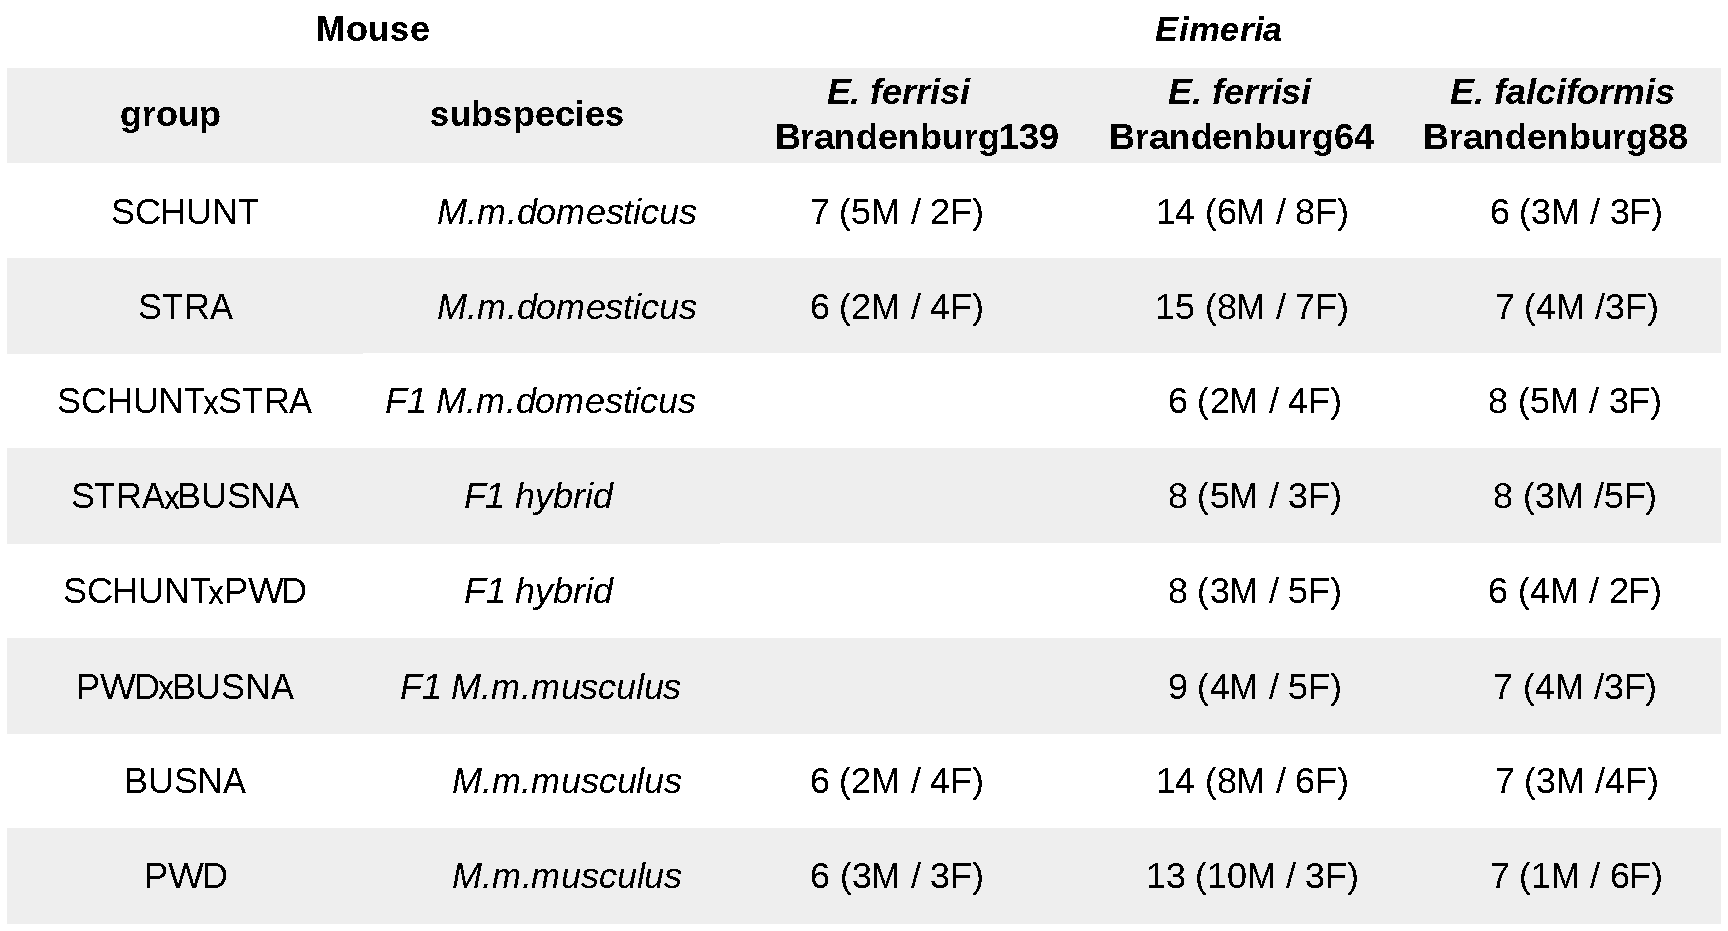
\includegraphics[width=\linewidth,height=\textheight,keepaspectratio]{images/Table1_final.pdf}
	\captionsetup{labelformat=empty}
	\caption{\textbf{Table 1.} Infection experiment design.}
\end{figure}
\addtocounter{figure}{-1}

\begin{figure}[H]
	\centering
	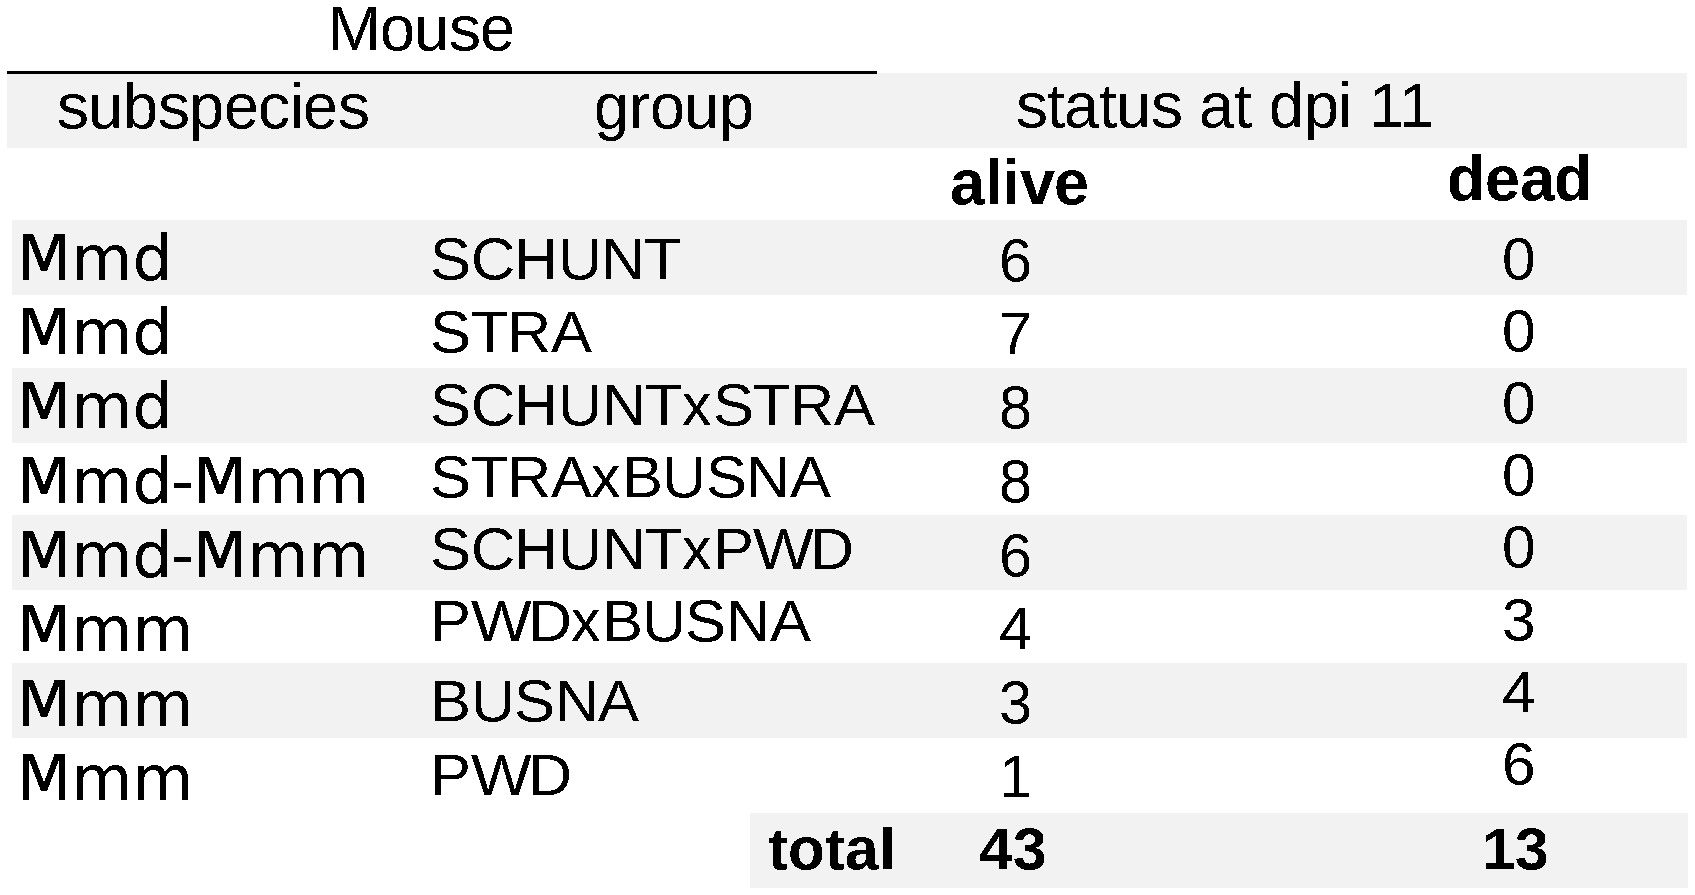
\includegraphics[width=\linewidth,height=\textheight,keepaspectratio]{images/Table2_final.pdf}
	\captionsetup{labelformat=empty}
	\caption{\textbf{Table 2.} Contingency table: number of mice and status at dpi 11 for each mouse group upon infection with \textit{E. falciformis} isolate Brandenburg88.}
\end{figure}
\addtocounter{figure}{-1}

\section*{Figures legends}

\textbf{Figure 1. Parasite isolates and mouse wild-derived strains.} (A) Map showing locations at which mice were collected for breeding of mouse strains and isolation of parasites. The purple line is an estimation of the center of the house mouse hybrid zone between \textit{M.~m.~domesticus} and \textit{M.~m.~musculus} based on sampling and genotyping of mice in this area \citep{Balard2020, dureje_mouse_2012, macholan_widespread_2019}. (B) The eight mouse groups (parents and F1s) used in our experimental infections.

\textbf{Figure 2. Parasite density (A) and relative weight (B) during \textit{Eimeria} infection.} Parasite density is calculated as number of oocysts detected (in millions) per gram of feces, relative weight is calculated as the percentage of weight compared to day 0. Mean and 95\% CI are plotted for each parasite isolate. All mouse groups are pooled together.

\textbf{Figure 3. Comparison of resistance, impact on weight and tolerance between mouse strains for both \textit{Eimeria~ferrisi} isolates.} (A) Maximum oocysts per gram of feces used as a proxy for (inverse of) resistance; (B) Impact on host health measured as the maximum weight loss during patent period relative to starting weight (\%); (C) Tolerance estimated by the slope of the linear regression with null intercept modelling maximum relative weight loss as a response of maximum oocysts per gram of feces. A steep slope corresponds to a low tolerance. We did not detect (A) either higher parasite shedding of the Eastern parasite isolate in Eastern mouse strains and vice versa or (C) higher tolerance of Eastern hosts infected by Eastern parasite isolate and vice versa, thus our results do not support the hypothesis of local adaptation between \textit{E.~ferrisi} and its host.

\textbf{Figure 4. No indication of resistance-tolerance coupling for \textit{E.~ferrisi} isolate Brandenburg64.} Colors represent mouse subspecies (blue: \textit{M.~m.~domesticus}, red: \textit{M.~m.~musculus}, purple: Mmd-Mmm). Left side: comparison of maximum oocysts per gram of feces used as a proxy for (inverse of) resistance (A), impact on weight measured as the maximum weight loss during patent period relative to starting weight (B) and tolerance between mouse groups estimated by the slope of the linear regression with null intercept modelling maximum relative weight loss as a response of maximum oocysts per gram of feces, a steep slope corresponding to a low tolerance (C). Maximum number of OPG and relative weight loss differ between mouse groups, but tolerance is similar. Right side: non significant positive correlation between mean maximum oocysts per gram of feces and mean relative weight loss (D) and absence of correlation between maximum oocysts per gram of feces used as a proxy for (inverse of) resistance and tolerance (E); Grey error bars represent 95\% confidence intervals. Our results do not support coupling between resistance and tolerance \textit{E.~ferrisi} isolate Brandenburg64.

\textbf{Figure 5. Coupling between resistance and tolerance for \textit{E.~falciformis} isolate Brandenburg88.} Colors represent mouse subspecies (blue: \textit{M.~m.~domesticus}, red: \textit{M.~m.~musculus}, purple: Mmd-Mmm). Left side: comparison of maximum oocysts per gram of feces used as a proxy for (inverse of) resistance (A), impact on weight measured as the maximum weight loss during patent period relative to starting weight (B) and tolerance between mouse groups estimated by the slope of the linear regression with null intercept modelling maximum relative weight loss as a response of maximum oocysts per gram of feces, a steep slope corresponding to a low tolerance (C). Maximum number of OPG, relative weight loss and tolerance differ between mouse groups. Right side: non significant negative correlation between mean maximum oocysts per gram of feces and mean relative weight loss (D) and strong negative correlation between maximum oocysts per gram of feces used as a proxy for (inverse of) resistance and tolerance (E); Grey error bars represent 95\% confidence intervals. Our results support coupling between resistance and tolerance \textit{E.~falciformis} isolate Brandenburg88.

\section*{Figures}

\begin{figure}[H]
	\centering
	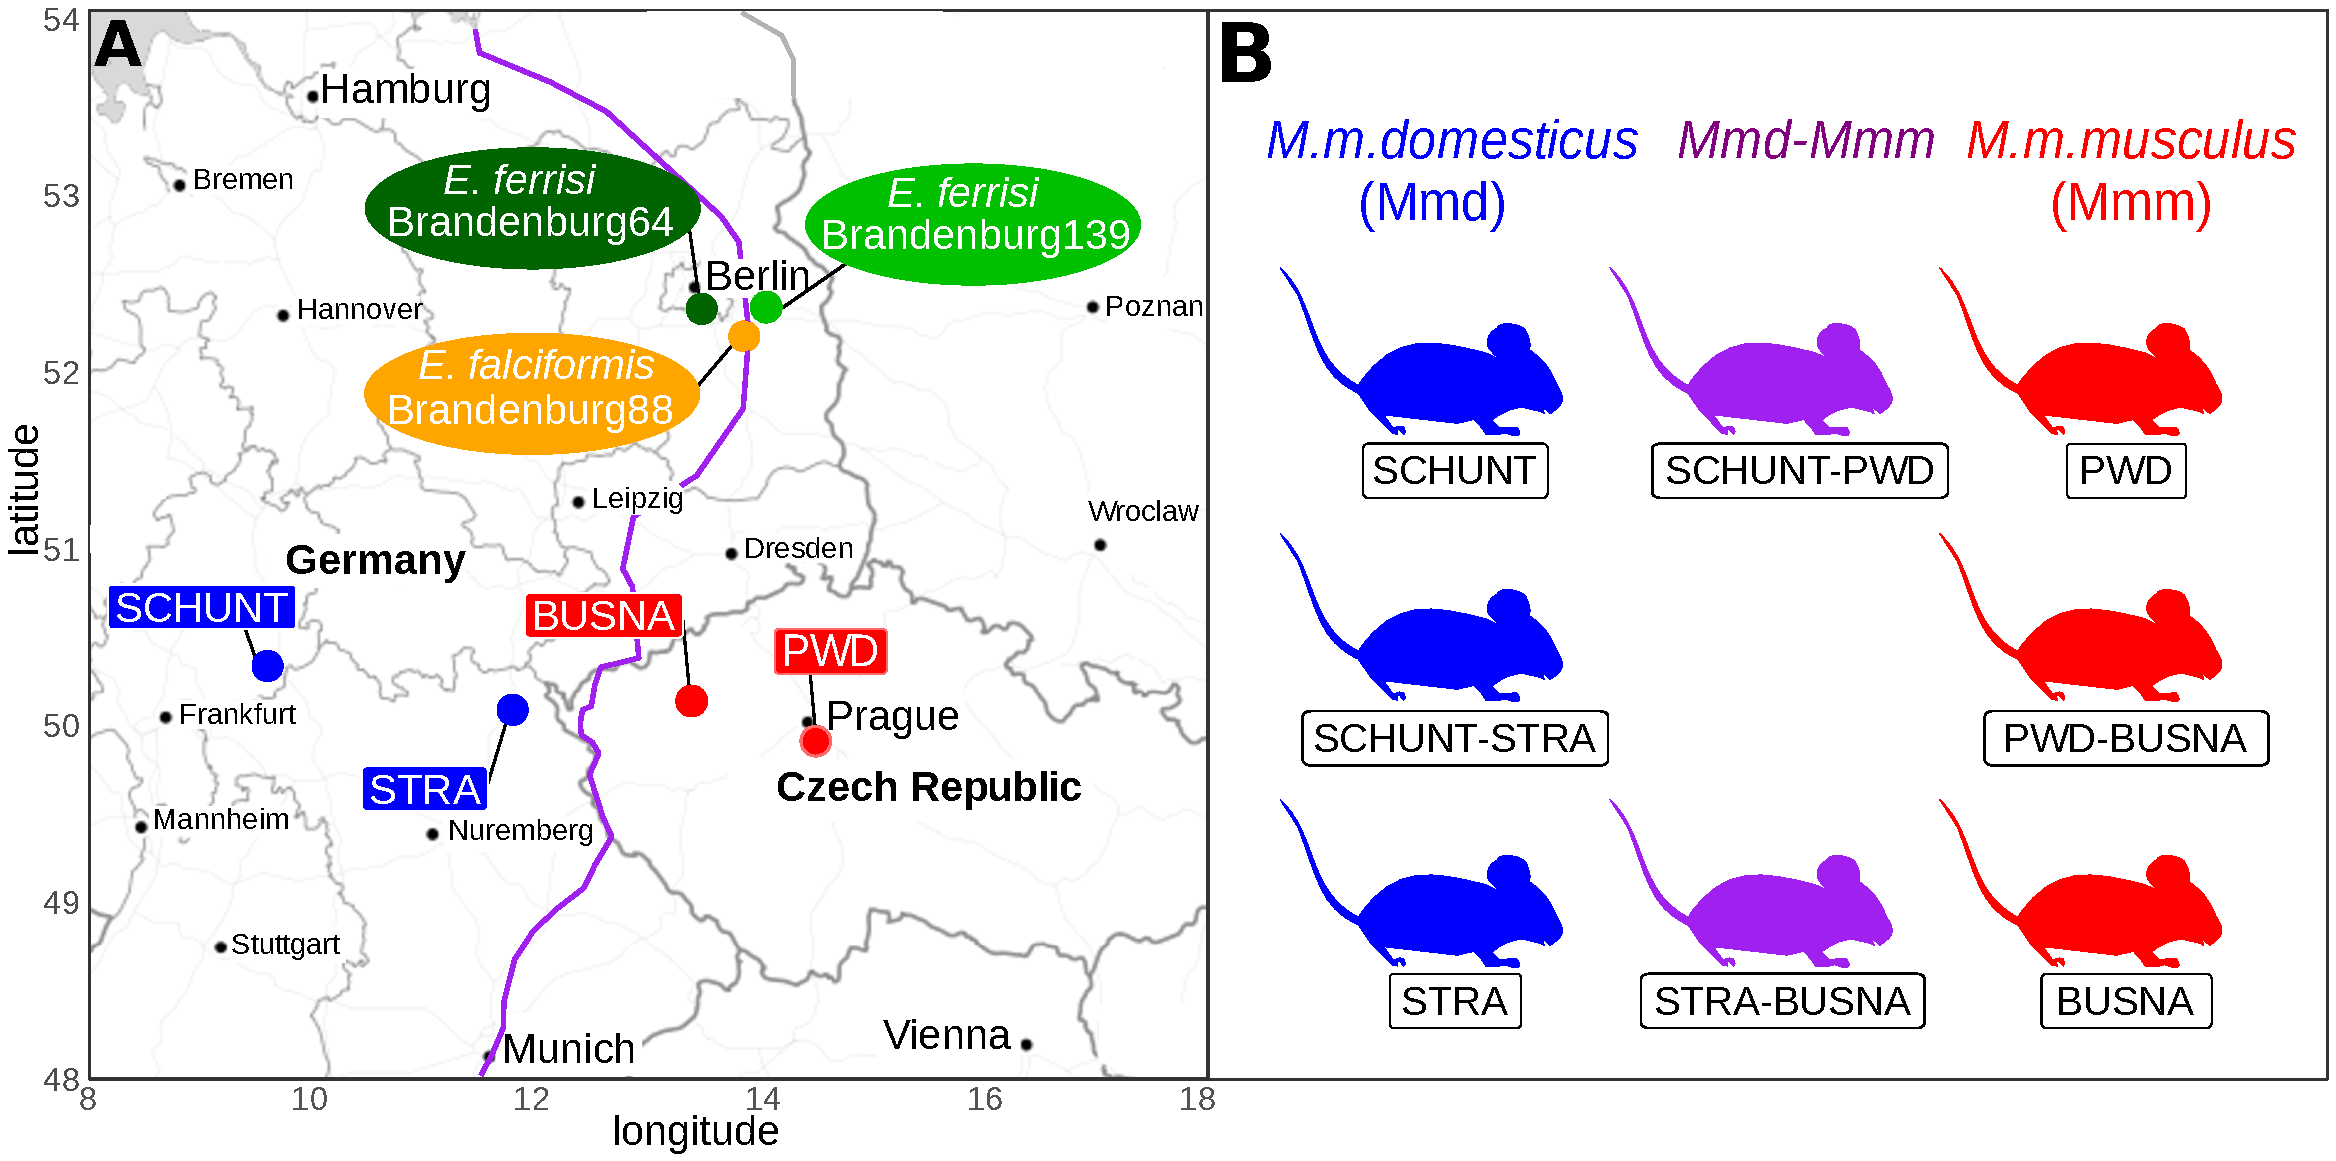
\includegraphics[width=\linewidth,height=\textheight,keepaspectratio]{images/Fig1_final.pdf}
	\caption{Parasite isolates and mouse wild-derived strains.}
\end{figure}

\begin{figure}[H]
	\centering
	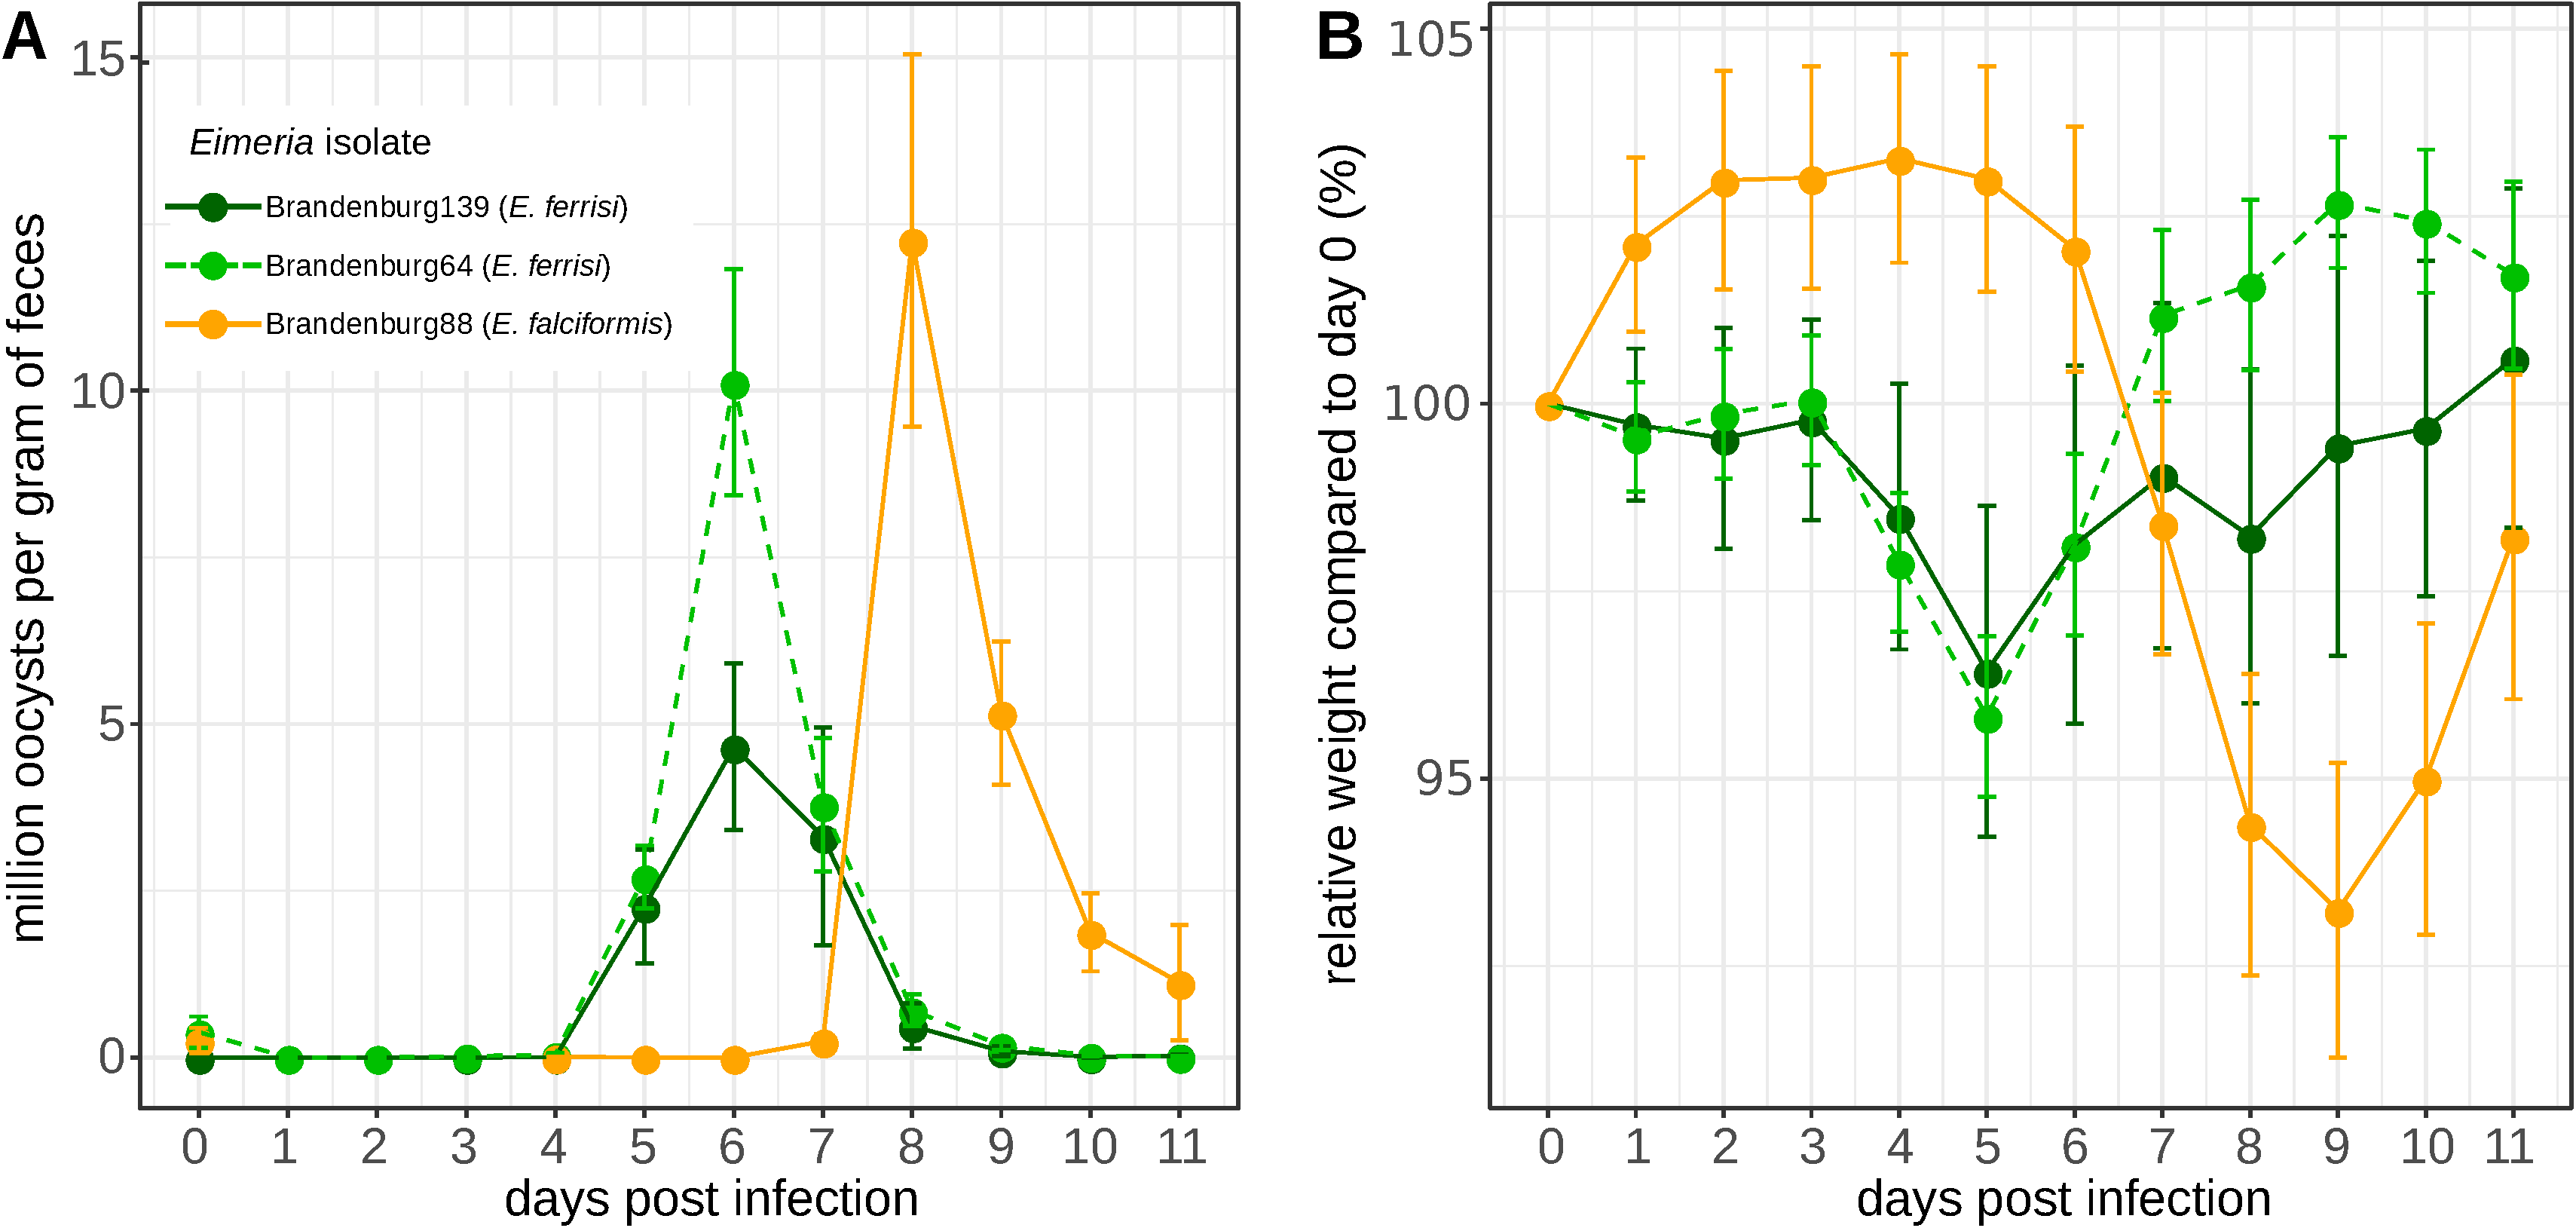
\includegraphics[width=\linewidth,height=\textheight,keepaspectratio]{images/Fig2_final.pdf}
	\caption{Parasite density (A) and relative weight (B) during \textit{Eimeria} infection.}
\end{figure}

\begin{figure}[H]
	\centering
	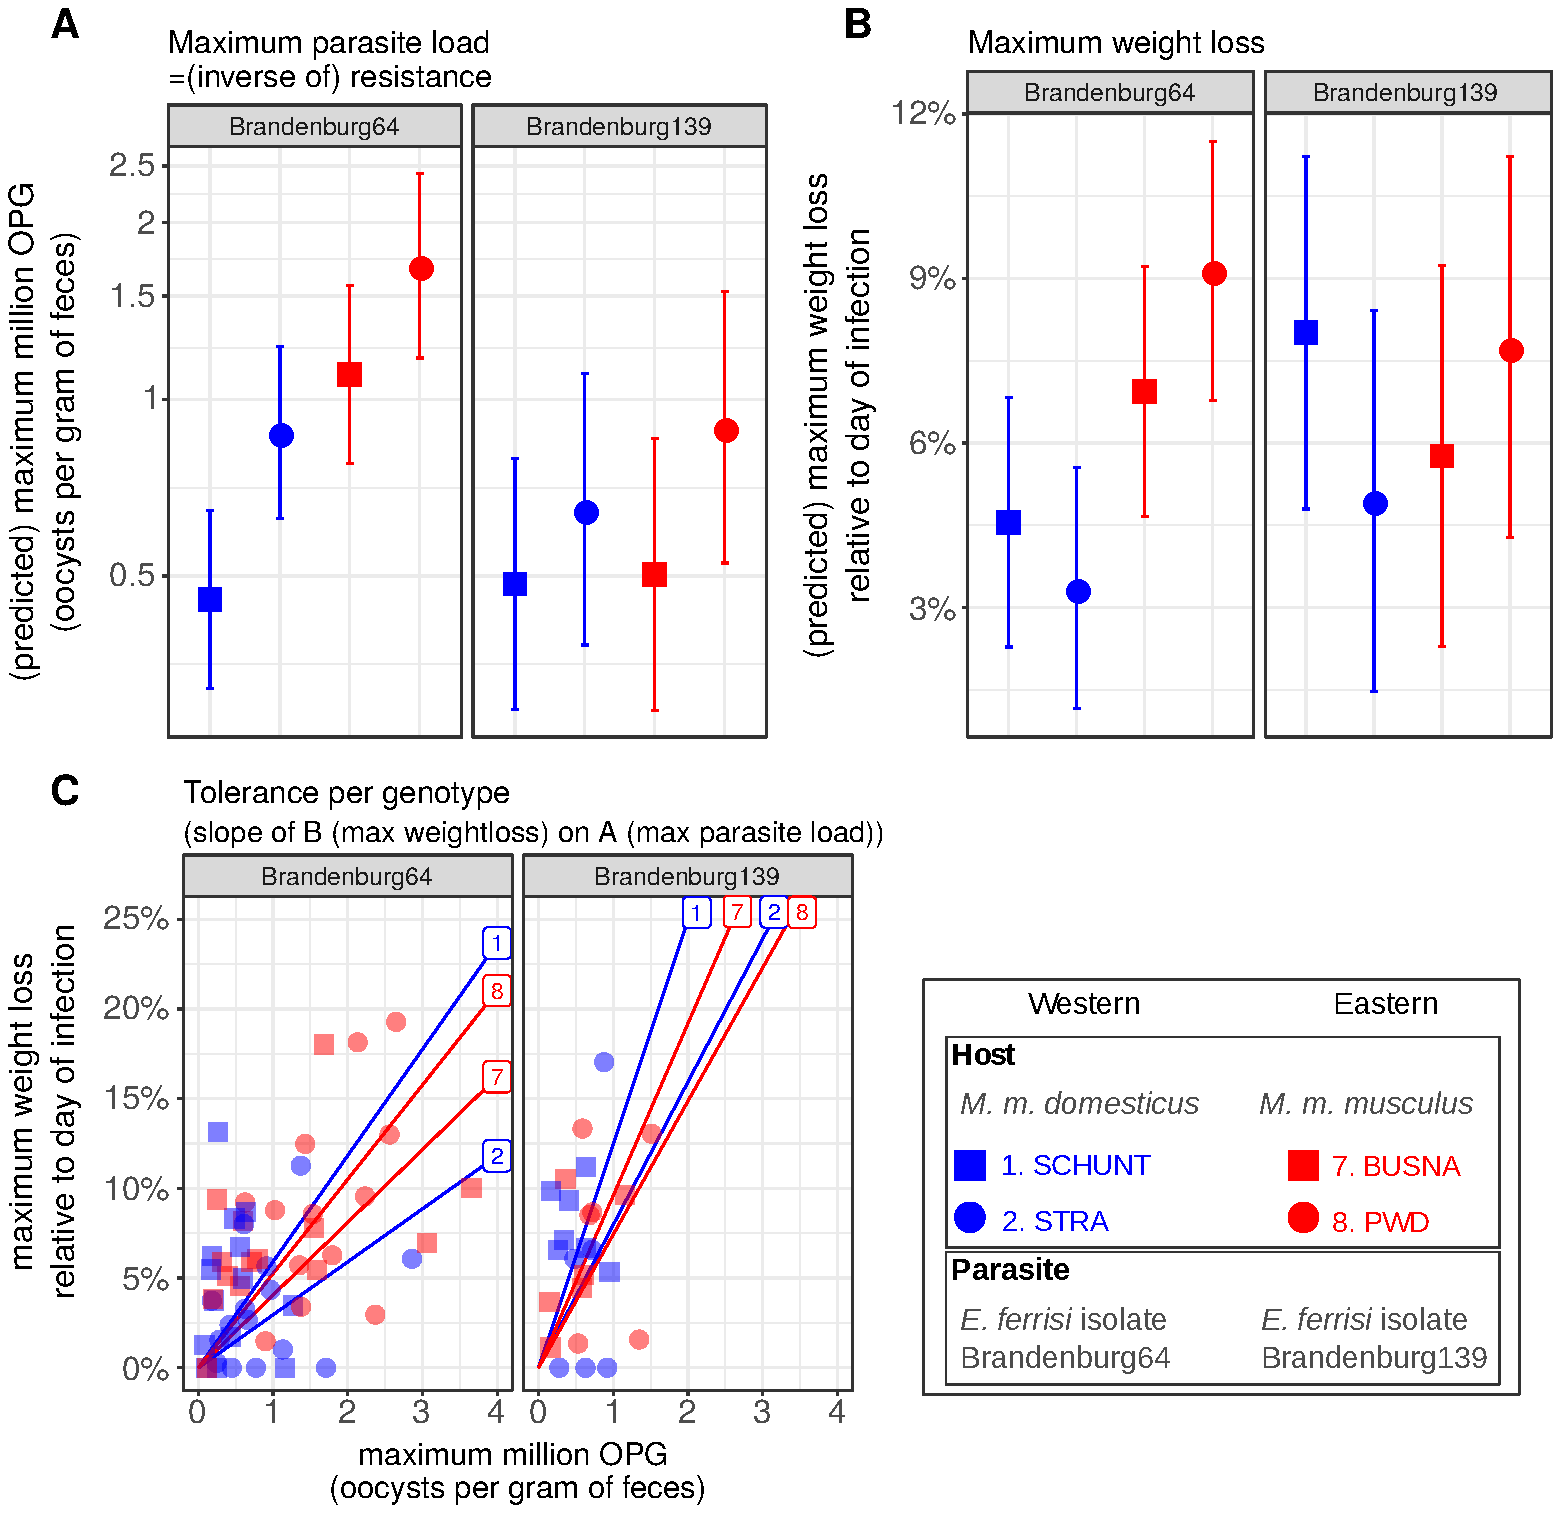
\includegraphics[width=\linewidth,height=\textheight,keepaspectratio]{images/Fig3_final.pdf}
	\caption{Comparison of resistance, impact on weight and tolerance between mouse strains for both \textit{Eimeria~ferrisi} isolates.}
\end{figure}

\begin{figure}[H]
	\centering
	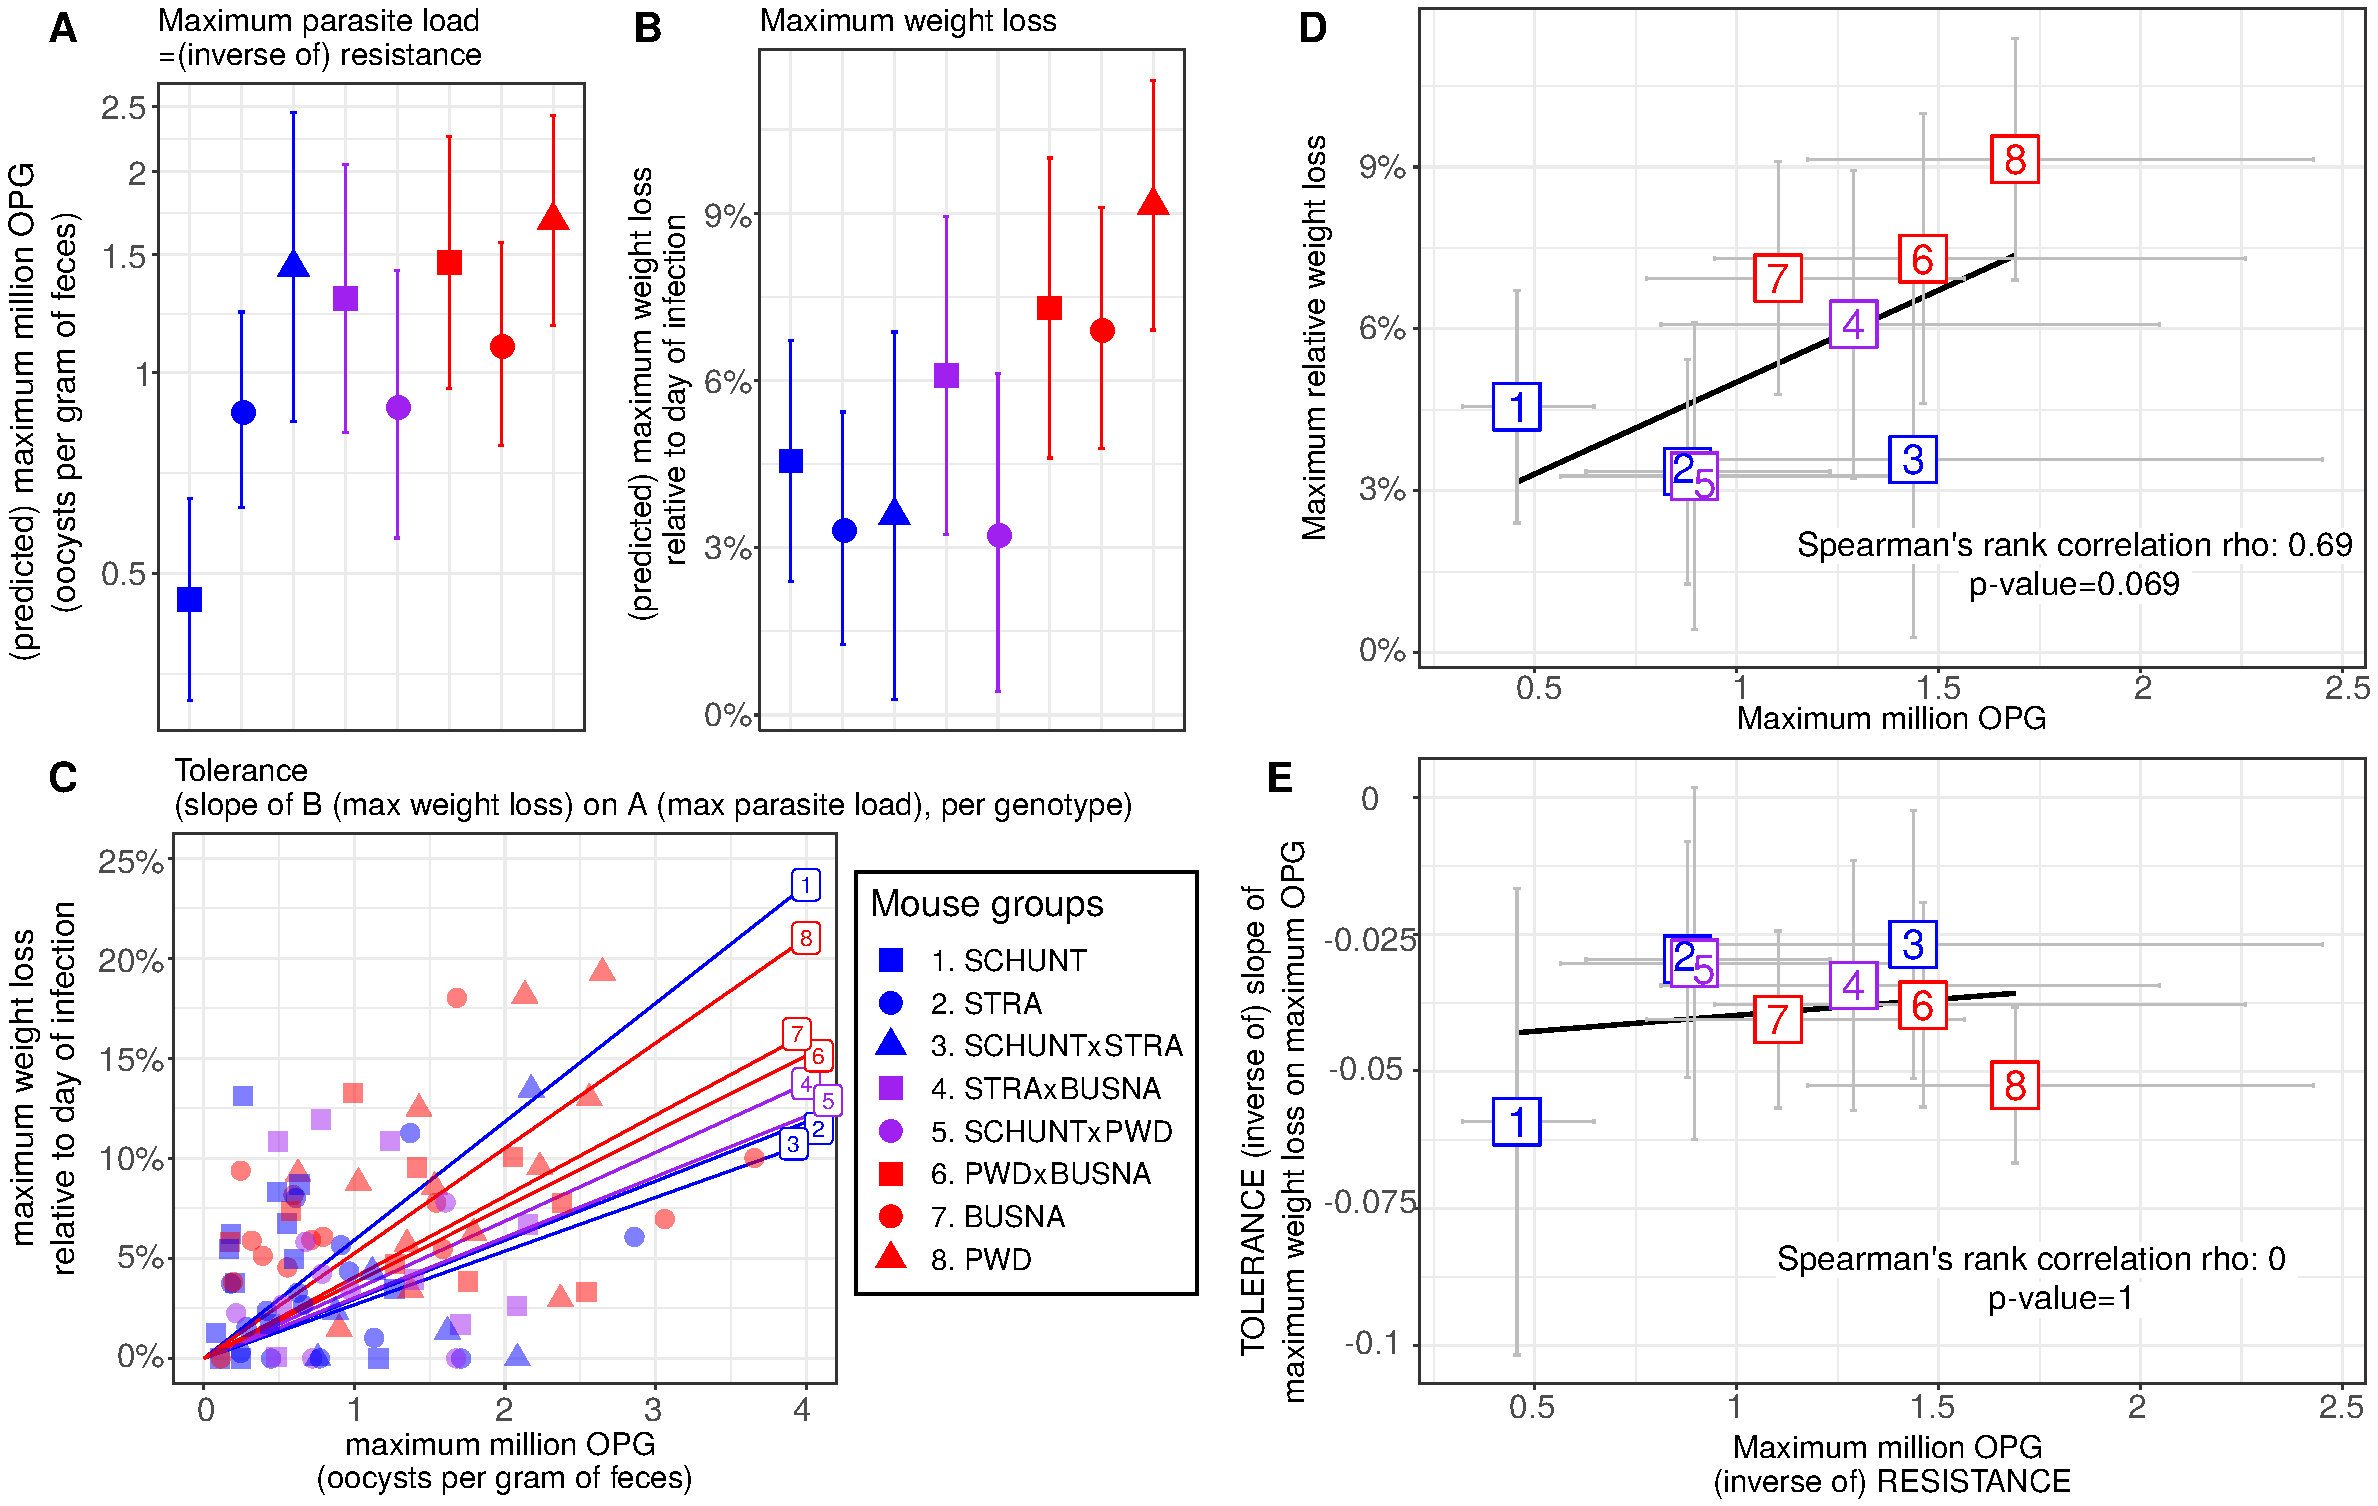
\includegraphics[width=\linewidth,height=\textheight,keepaspectratio]{images/Fig4_final.pdf}
	\caption{No indication of resistance-tolerance coupling for \textit{E.~ferrisi} isolate Brandenburg64.}
\end{figure}

\begin{figure}[H]
	\centering
	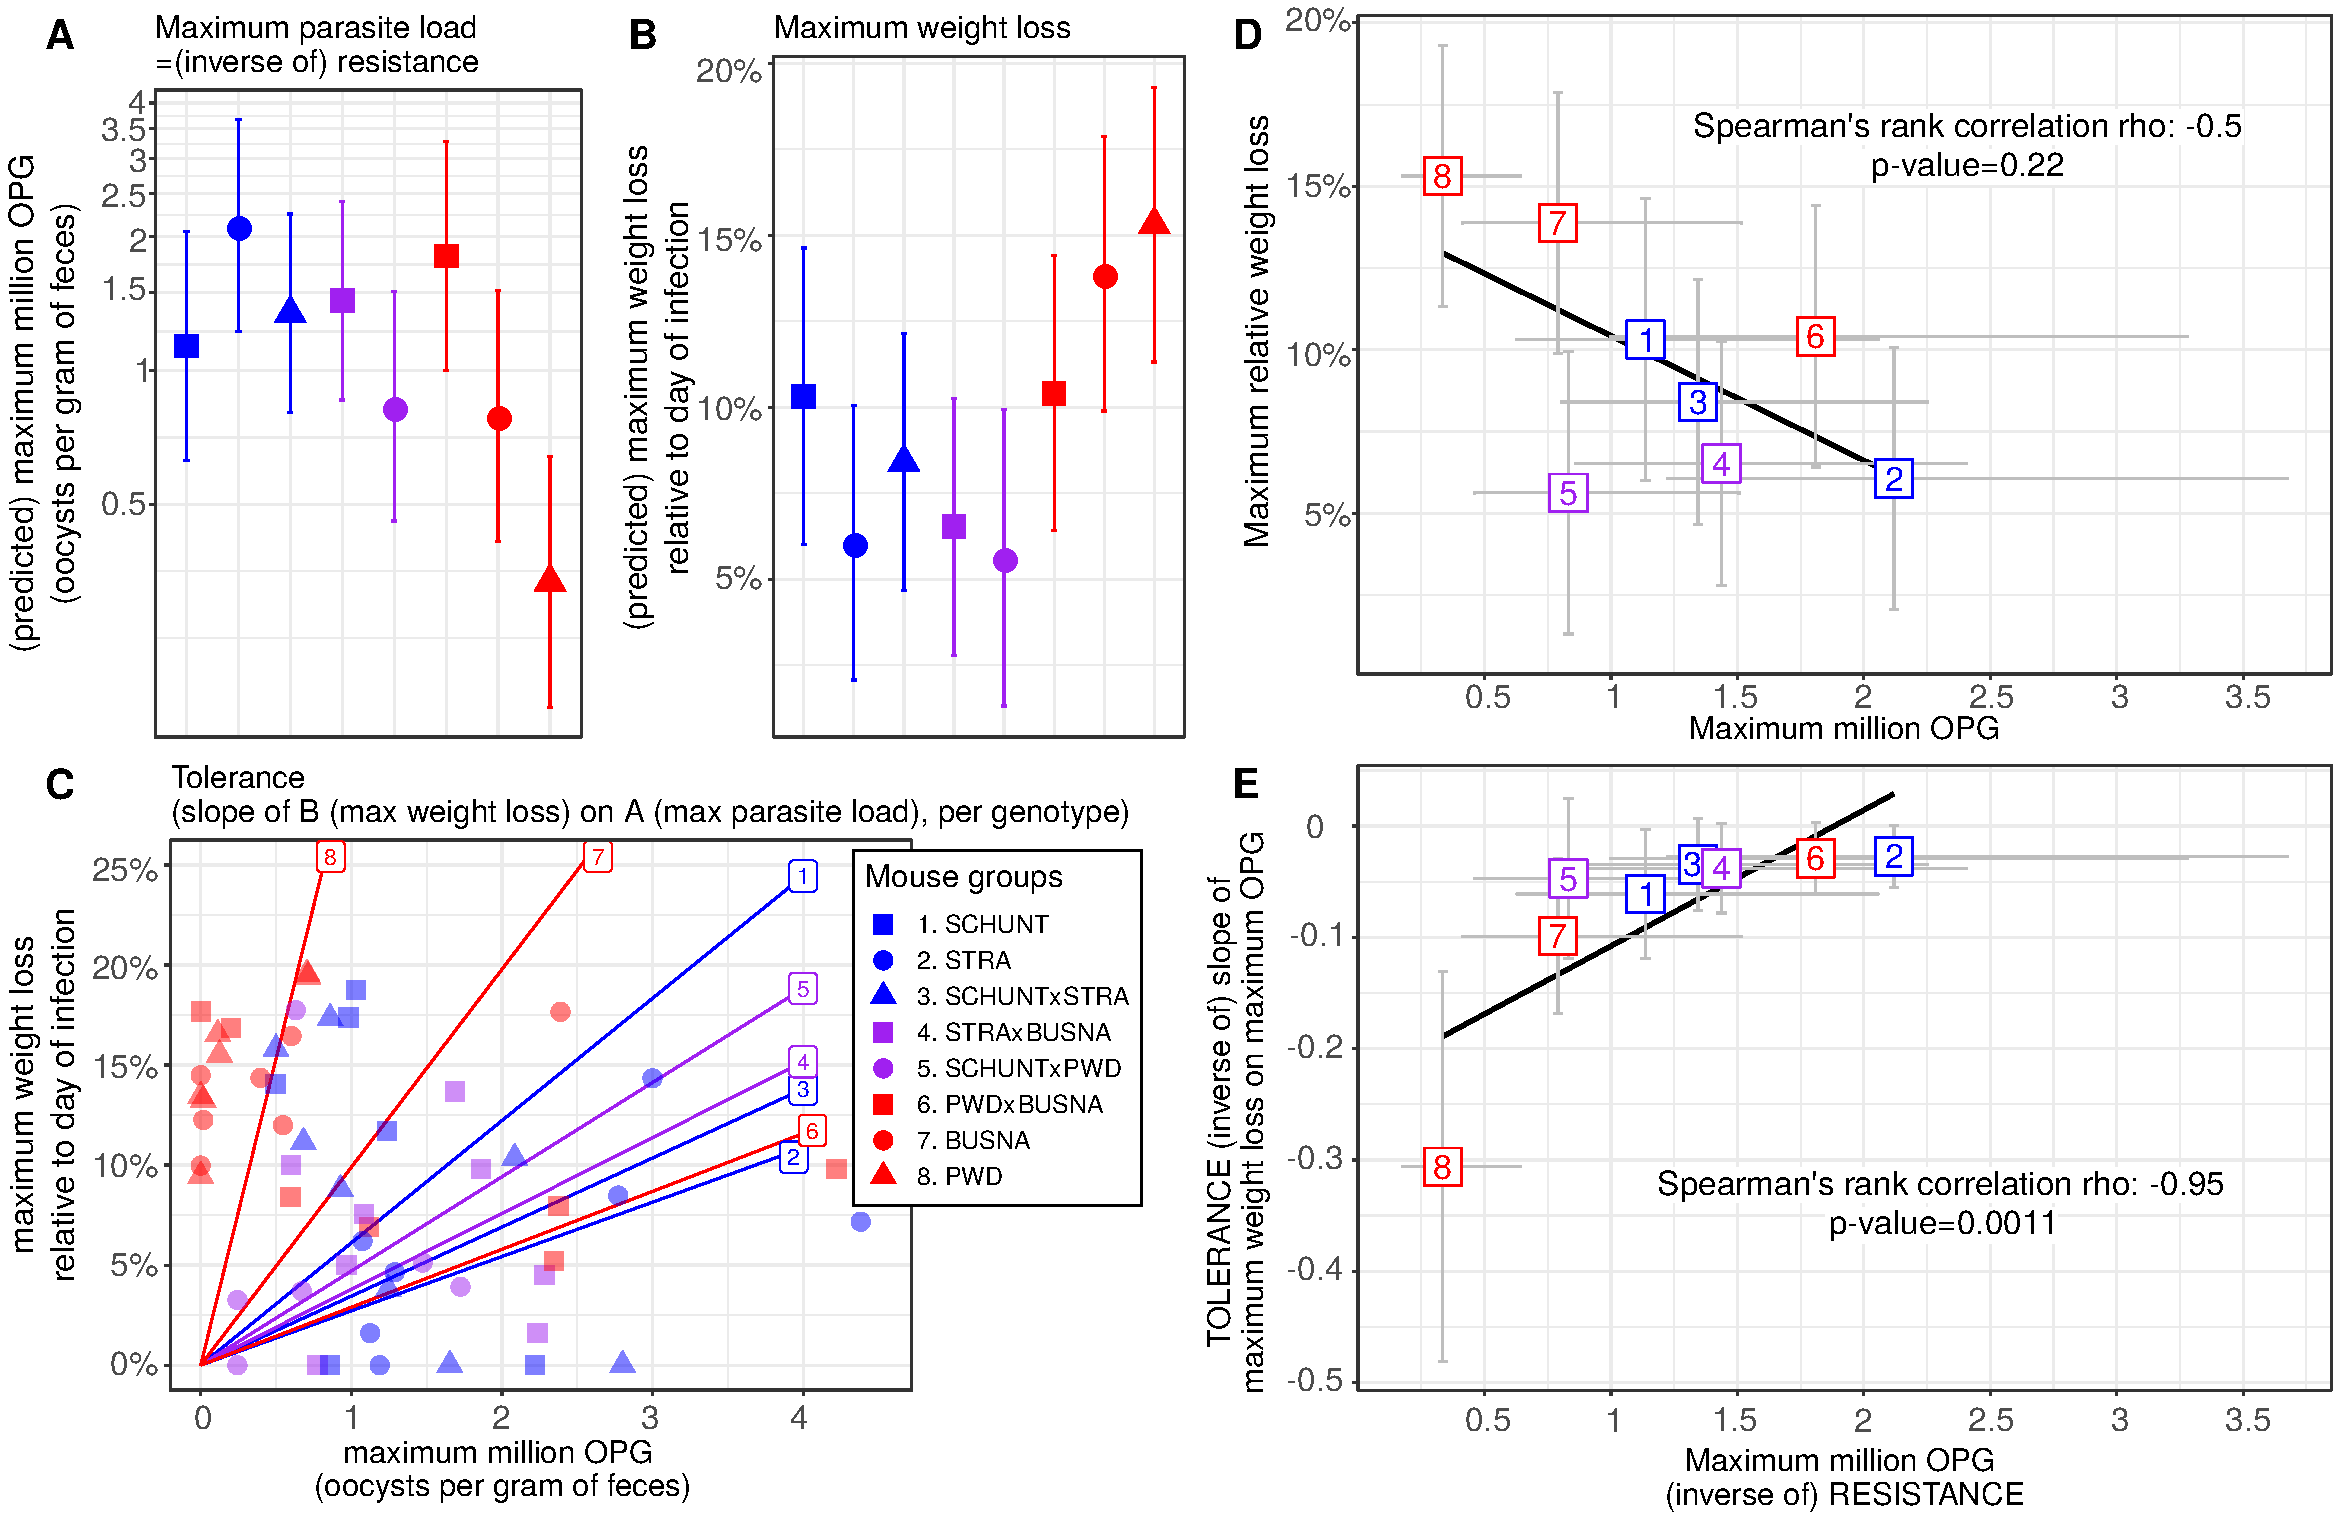
\includegraphics[width=\linewidth,height=\textheight,keepaspectratio]{images/Fig5_final.pdf}
	\caption{Coupling between resistance and tolerance for \textit{E.~falciformis} isolate Brandenburg88.}
\end{figure}

\end{document}
